\chapter{Unity framework}
The purpose of this chapter is to describe the Unity framework used to automate game testing. 
The framework used is an extension of initially developed by Ballabio \cite{ballabio_framework} capable of running automated 1 vs 1 matches on dynamically loaded maps between bots with configurable parameters.

\section{Motivation for the framework}
%TODO
Academic research on map generation for FPS is still newborn and there isn't yet a consensus on the tools to use. Most researches followed the example from Cardamone and used Cube 2: Sauerbraten as their starting engine, later customized to fit the needs of the research. Others, for example Bhojan Anand and Wong Hong Wei in \cite{bhojan_hong_arena}, opted to create their own game engine, a complex tasks which doesn't really pay off if used for a single research.

Given that game development has evolved in the years and it's now easier to code games using more modern tools and engines, for example Unity\footnote{https://unity.com/} or Godot\footnote{https://godotengine.org/}, it should be now feasible to produce a new, rather generic framework that can be easily customized to adapt it to any possible research one wants to conduct.

For this reason in his thesis Ballabio \citep{ballabio_framework} developed a new Unity framework which offers a plethora of useful capabilities for any kind of experiment, most notably the possibility of building and embedding the game in a web page, allowing researches to gather data from users playing from anywhere in the world, without requiring any complex installation or setup on their machines.

However, Ballabio's framework had a big shortcoming in the lack of bots, an essential tool to run any kind of simulation required by many techniques, such as Search Based Procedural Content Generation. Bots have been introduced with our work in this thesis and will be described in \Cref{section:unity_bots}.

\section{High-level overview}
In order to help readers follow through the explanation of our study, a small overview of Ballabio’s framework main concepts is given below. For more details readers are advised to consult \cite{ballabio_framework}.

\subsection{Map representation}
Maps are structured as grids of orthogonal tiles and are internally represented by matrices of characters, where each cell corresponds to a specific tile. Each tile can represent either an empty space, a wall, an ammo pack, a medkit, a spawn point or stairs. 
In case the map has multiple floors, each floor is represented by one such matrix of characters. An example of map can be seen in \Cref{fig:char_map}.
Independently from how a map is initially represented (e.g. all-black, cellular, …), it must always be converted to this format.

\begin{figure}[hbtp]
\centering
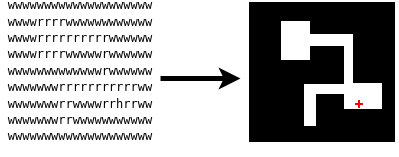
\includegraphics[width=0.7\linewidth]{Images/images/charmap.drawio.png}
\caption{Mapping of matrix representation of the actual map. The black areas are non-walkable spaces, the '\textcolor{red}{\textbf{+}}' is a medkit.}
\label{fig:char_map}
\end{figure}


\subsection{Game manager}
The \textbf{Game Manager} is the module responsible for the overall behavior of a match. Different implementations of \textit{Game Manager} exist, each representing a different type of match and handling its entire life cycle, from setup to the final scoring.

\subsection{Map Manager}
The \textbf{Map Manager} controls the generation or the import and the assembly of the map and the displacement of objects inside it.

For the generation of the maps and displacement of spawn points and pickups it uses the \textit{Map Generator}, of which various versions exist depending on the specific generation algorithm (e.g. digger), while for the conversion from text representation to the final 3D map the \textit{Map Assembler} is employed.

\subsection{Experiment manager}
The \textbf{Experiment Manager} is a stand alone module that allows to create and manage the experiments used to perform user-based validation. Once an experiment has been defined, the \textit{Experiment Manager} automatically assigns to the users the matches to play and collects the desired information.
Given that our research doesn’t involve any interaction with the user, we didn’t use any \textit{Experiment Manager} in our project.

\subsubsection{Entities}
The \textbf{entities} are the agents that take part in a match.
In their most basic form, an \textit{entity} essential parameters are its position, health and weapons. Given that one of the focus of our project was implementing an AI in the game, entities will be described more in \Cref{section:unity_bots}.

\subsubsection{Weapons}
Any kind of firearm used by entities, defined by parameters such as their type (raycast, projectile, laser), damage, projectiles per shot, reload time, …

\subsubsection{Game modes}
Ballabio’s framework supports 3 different kinds of mode, \textit{Duel}, \textit{Target Hunt}, \textit{Target Rush}. For the purpose of our research, we focused only on \textit{Duel}, which represents a simple 1-vs-1 deathmatch with respawn.

\section{Data gathering and processing}
To perform any kind of experiment, we need to be able to gather data from various matches for further processing. 

Our framework is capable of saving a lot or raw data coming from matches. This data is then analysed outside of Unity to extract some interesting metrics. In the following sections we will describe the data gathered and how it is processed.

\subsection{Match raw data}

For every match, the framework gathers the following data, which measures characteristics determined by the map topology:

\begin{itemize}
\item \textit{Time to engage}: Measures the time between the end of a combat event and the next one, or, right at the beginning of the match, between the respawn time and the first combat start.
\item \textit{Time in fight}: Measure the total time a bot spends fighting an enemy, considering also the time spent searching it right after losing its tracks.
\item \textit{Number of fights}: Total number of fights.
\item \textit{Time between sights}: Total time between the moment an entity can no longer detect an enemy and the moment it is detected again, considered for every fight event.
\item \textit{Number of sights}: Number of time an enemy return sighted after becoming undetected.
\item \textit{Time to surrender}: Time between the moment a bot loses track of the enemy and the moment it decides to abort searching for it.
\item \textit{Number of retreats}: Number of times a bot abandons searching an enemy after a fight.
\end{itemize}

Additionally, for each entity in the game, the following data is measured:

\begin{itemize}
\item \textit{Frags}: Number of kills performed by the entity
\item \textit{Deaths}: Number of deaths of the entity.
\item \textit{Shots}: Number of bullets fired by the entity.
\item \textit{Hits}: Number of times a projectile shot by the entity hit an entity (including itself).
\end{itemize}

\subsection{Analysis metrics}
By taking inspiration from some of the factors that experts in the field identified as required for the creation of good maps (\cite{game_design_secret_sages, best_multiplayer_maps_one, best_multiplayer_maps_two}), we selected some metrics measuring interesting aspects during the design of levels.

\subsubsection{Balance}
Map balance, interpreted as the possibility offered by the map to achieve a fair match between participants, is possibly the most important characteristic to observe, especially for multiplayer games. While balancing could be obtained by simply using symmetrical maps (as done in \textit{Splatoon}\footnote{Nintendo, 2015}), a good, balanced map should offer a good balance between advantage and disadvantage situations in order to allow each side to contrast the others.
Weapons usually offer a significant tactical advantage versus others in some specific situations. Shotguns for example are better suited for short-range combat, while sniper rifles excel at long-range. Map structured in specific ways could therefore favour only a single type of game style. 
An effective way to measure the efficiency of a player is by computing the kill/death ratio: the best players are those that can kill others without attracting too much enemy fire.
To evaluate the balance we opted to use the \textbf{entropy} of all kills, used by both Stucchi \cite{stucchi_evoluzione} and Arnaboldi \cite{arnaboldi_framework} to generate balanced maps.

\begin{equation}
entropy = \sum_{i=1}^{n} - \left( \frac{k_i}{k_{tot}} \right) \log_2 \left( \frac{k_i}{k_{tot}} \right)  
\label{eq:entropy}
\end{equation}

In formula \eqref{eq:entropy} $k_i$ represents the number of frags of the i-th bot, while $k_{tot}$ is the total number of frags in a match.
Entropy values vary in the the [0-1] range: values close to zero indicate a wildly unbalanced match in which a player trumped all the others, while values close to 1 represent balanced matches.

\subsubsection{Pace}
Another important aspect of matches to keep track of is frequency of encounters between players. Matches which evolve too slowly, with very few battles between sides, would result boring and not particularly engaging. On the contrary, too high frequency encounters would make players feel overwhelmed and would prevent any sort of tactic, making the experience frustrating.
To compute a \textit{pace} value normalized in the [0,1] interval the following function \Cref{eq:pace} was used.

\begin{equation}
pace = 2 * \frac{1}{1 + exp \left( -5 * \frac{NumberOfFights}{\sum TimeToEngage} \right) } - 1
\label{eq:pace}
\end{equation}

The sigmoid function \Cref{eq:pace} computes values for \textit{pace} close to 0.9 for average time to engage equal to 3 seconds. %TODO verify number

%TODO add other metrics in case they are needed

\subsection{Performance metrics}
Besides metrics measuring characteristics of the map, it's useful to keep track of other metrics regarding the performance of the different bots during matches.
The metrics we extract are:
\begin{itemize}
\item \textbf{Number of Frags} Total number of frags in a match.
\item \textbf{Accuracy} How precise each bot is when shooting, calculated as the ratio between the number of \textit{Hits} and the number of \textit{Shots}.
%TODO missing metrics from Arnaboldi
\end{itemize}

%TODO not sure whether all the metrics above are ever used, so we can probably not describe them for the time being.


\section{Unity bots} \label{section:unity_bots}
In this section we'll be analyzing the bots we developed for our research. We will first be briefly discuss their architecture and later focus our attention on how they work by studying one of their processing cycles. 

\subsection{Bot architecture}
The AI of the bots we developed is structured as a modular system, composed of four distinct layers, each with its own specific responsibilities. This design, which can be seen in \Cref{fig:modular_layered_bot} allows for a clear division of responsibilities and ease of maintenance, as changes can be made to individual layers without affecting the entire system.

\begin{figure}
\centering
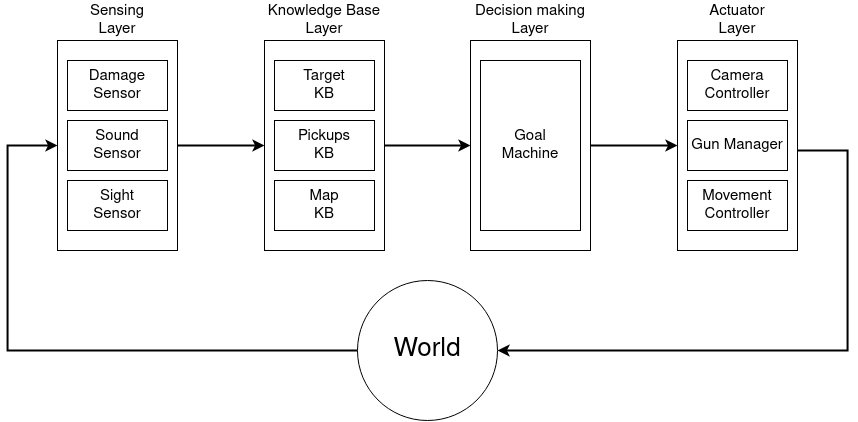
\includegraphics[width=0.8\linewidth]{Images/images/LayeredArchitecture.drawio.png}
\caption{Bot layered architecture and information flow between the layers and the world.}
\label{fig:modular_layered_bot}
\end{figure}

The \textbf{Sensing layer} is one of the two interfaces the bot has with the in-game world and it is in particular responsible  of receiving inputs from the environment in order to provide access to this information to the following layer. Examples of data sensed by this layer are sounds from guns firing, damage received by the bot and visual information such as the visibility of an item or entity.

The \textbf{Knowledge Base layer} is responsible for storing and processing all relevant information about the game world, both learned through \textit{sensing} and given as initial domain knowledge. This layer acts as a repository of information that the bot can use to make informed decisions. The information provided by the \textit{Knowledge Base} can include last known locations of enemies, the shortest paths to different destinations, the location, estimated activation time and effectiveness of different pickups and so on. By using this information, the bot can make informed decisions and execute effective strategies within the game.

The \textbf{Decision Making layer} is responsible for determining the objectives and action plans for the bot based on the (perceived) current state of the environment and the bot itself. This layer evaluates various options and chooses the one that is most likely to lead to success, given the information available from the \textit{Knowledge Base}. Examples of decisions made in this layer include whether to attack or flee from an enemy; whether to track a lost enemy or instead collect health or ammo supplies and so on. The \textit{Decision Making layer} continuously strives to maximize the bot chances of success by carefully weighing the potential outcomes of each available action.

Finally, the \textbf{Actuator layer} is responsible for executing the actions determined by the \textit{Decision Making layer}, translating them into actual in-game interactions such as moving around, rotating the view, shooting, reloading, and switching weapons, which ultimately allow the bot to interact with the virtual world.

A more in-depth description of how the different tasks of each layer are handled is provided in the following sections.

\subsection{Sensing layer}
The \textit{Sensing layer} purpose is to receive raw data from the world in order to allow other layers to process it.
It important to notice that this layer only checks if an event happens, other layers are then responsible to understand if the bot should react to such event. This means, for example, that an enemy being visible according to the \textit{Sight sensor} doesn’t necessarily mean that the bot can/should immediately react to it; rather, upper layers will usually introduce some delay to simulate reaction time of a normal human.

The \textit{Sensing layer} is composed of three different modules.

\subsubsection{Sight sensor}
Takes care of determining whether a given location, item or entity is currently visible by the bot, based on three criteria:
\begin{description}
\item[Presence of obstacles] If an obstacle, such as a wall, ceiling or other entity fully covers the target, then it won't be considered visible. In order to check this, the Unity raycast function is employed.
\item[Bot field of view] If the target is outside the cone of vision of the bot, then it's not visible;
\item[Bot depth of view] If the target is too far away, the bot won't be able to see it.
\end{description} 
%TODO image about sight, hear

\subsubsection{Sound sensor}
The \textit{Sound Sensor} is responsible for detecting and determining the origin of sounds in the game world. Currently, the only source of noise in the game is gun fire, whose volume depends on the type of weapon fired. Then, depending on the distance of the sound source and the sensitivity of the bot, the bot might detect or not that a shot was fired.
%TODO image about sight, hear


\subsubsection{Damage sensor}
Finally, the \textit{Damage sensor} takes care of detecting whether an entity received damage recently.


\subsection{Knowledge Base layer}
The \textit{Knowledge Base layer} purpose is analyzing data received from the \textit{sensing layer} and, combined with knowledge of the world provided in advance, provide tactical information to be used by the \textit{Decision layer}.
There are three modules in this layer.

\subsubsection{Target knowledge base}
\label{subsubsection:target_knowledge_base}
The \textit{Target Knowledge Base} module is responsible for determining the presence and position of enemies according to the bot. 
Before understanding exactly how this component works, it's crucial to understand the difference between a visible target and a detected target.
 
A visible target is one that is currently visible to the bot based on the information provided by the \textit{Sight Sensor}. 

A detected target, on the other hand, is one that has been visible for a sufficient amount of time that the bot can react to its presence and will continue to remain detected until after a while it is no longer visible. 

By allowing enemies to be visible, but not detected according to the knowledge base, it is possible to emulate reaction delays of a typical human player.

According to the \textit{Target Knowledge base}, a target can be in three different states:
\begin{description}
\item[Detected] The target recently remained visible for enough time for the bot to notice. The amount of time is inversely related to the distance of the target, so that the bot reacts faster the closer the enemy is\footnote{A more accurate analysis on reaction time and distance can be found in \cite{rabin_reaction_time}}.
\item[Lost] The target isn't currently detected, but was detected until recently.
\item[Undetected] The target isn't detected and wasn't considered detected recently.
\end{description}

Knowing whether an enemy is considered detected or not is crucial for upper layers to understand whether we know its exact location (when detected), can only approximate it (when lost) or if the whereabouts are unknown (when undetected).

\subsubsection{Pickup Knowledge Base}
%TODO

The \textit{Pickup Knowledge Base} keeps track of all the pickup items present in the map. Its main responsibilities are determining the location and effect of all pickups, as well as providing precise or estimated data about their past, present, and future status.

This last part is especially critical: since pickups become temporarily disabled after being collected, the knowledge base must be able to determine whether a bot can pickup something or not at any given time.

In order to do so, the \textit{Pickup Knowledge Base} internally keeps track of when the pickup was last seen, when it was last seen active and what is the latest estimated activation time. All this information is updated whenever a pickup is visible. 

Using this information to estimate activation times is pretty straightforward, in particular, if a visible pickup is currently active, then its status is obviously active, while in case it is disabled, the estimated activation time is computed as the current time plus half the normal pickup delay or the current estimated activation time, whichever is higher.

Additionally, if a bot recently collected a pickup, there is no need to estimate the next respawn time, it will be set to the normal pickup cool-down.

%TODO Maybe remove?
\subsubsection{Map knowledge base}
The \textit{Map Knowledge base} is used to keep track of when any specific area of the map was last visited. Keeping track of this information can help the bot decide what should be the next area to inspect or predict where an enemy might be located.

\subsubsection{Navigation system}
The \textit{Navigation system} is a critical component responsible of calculating the path of an agent to a given destination, keeping into account the topology of the map and any obstacle along the way. Without this component traversing the game map wouldn't be possible.

Currently, our \textit{Navigation system} relies on the Unity Navigation and path finding system\footnote{https://docs.unity3d.com/Manual/Navigation.html}.

\subsection{Decision making layer}
The \textbf{Decision Making layer} has the task of, given the current state of the bot and the environment, choose the objective that should be pursued and, as a consequence, the action plan to follow.

In order to obtain a rather flexible, yet easy to understand and maintain AI, we opted to mix together some of the decision making techniques discussed in \ref{subsection:theory_decision_making}, ultimately creating a fuzzy, state-based decision making system backed by action plans defined by behavior trees.

In our system, the bot has currently 4 possible states representing what the bot is currently trying to achieve: \textbf{Wander}, \textbf{Fight}, \textbf{Collect pickup} and \textbf{Search enemy}, which will be described in detail in the next sections.

No transition between these states is defined; rather, depending on the bot current status and knowledge, each state calculates a \textit{score} and at any time the state with the higher score is the current one. This system makes it possible for the bot to change its behavior as a response to any possible event without the need for the programmer to explicitly define this reaction, ultimately making it possible to add new states by simply defining their score function without having to worry about integrating this new state with the others.

Each state uses a behavior tree to define the sequence of actions that the bot will take to achieve the objective of the state itself. Using a graphical tool such as behavior trees makes it incredibly easy for everyone, even without programming knowledge, to visualize, modify and tweak the behavior of the bot in each of the states.

In order to simplify a little bit the visualization of the Behavior Trees, the various images presented in the next sections will separate between the action plan governing the momement of the bot and the action plan governing instead camera and guns.

For a detailed reference on the syntax used for Behaviour Trees, check \ref{section:unity_bots} in the Appendix.

\subsubsection{Wander}

\begin{figure}[hbtp]
\centering
\begin{subfigure}[c]{0.4\linewidth}
	\centering
	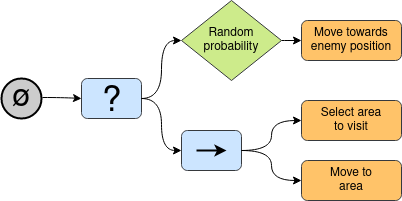
\includegraphics[width=\linewidth]{Images/images/WanderMovement.drawio.png} 
	\caption{Movement}
\end{subfigure}

\begin{subfigure}[c]{0.3\linewidth}
	\centering	
	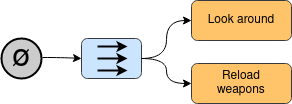
\includegraphics[width=\linewidth]{Images/images/WanderHead.drawio.png} 
	\caption{Camera and guns}
\end{subfigure}

\caption{Behaviour Trees governing the actions of the bot while wandering}
\label{fig:wander_bt}
\end{figure}

%
%\begin{figure}
%\centering
%\captionsetup[subfigure]{}
%\subfloat[\centering Movement]{
%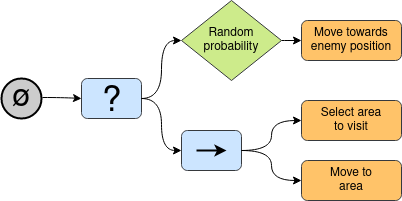
\includegraphics[width=0.3\linewidth]{Images/images/WanderMovement.drawio.png}} 
%
%\subfloat[\centering Camera and guns]{
%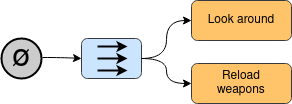
\includegraphics[width=0.4\linewidth]{Images/images/WanderHead.drawio.png}} 
%\caption{Behaviour Trees governing the actions of the bot while wandering}
%\label{fig:wander_bt}
%\end{figure}

When a bot is in \textit{Wander} state, pictured in \Cref{fig:wander_bt}, it has no specific objective, like collecting a pickup or chasing someone, and it will just roam around the map in the hope of stumbling upon the enemy. As such, this state tends to be a last resort and has therefore a very low score.

When wandering, a bot will constantly do three things in parallel:
\begin{itemize}
\item \textbf{Move around}: The bot will explore the map by selecting a random destination to reach, giving more preference to places not visited recently. In order to allow emulating skilled players, which might be able to estimate from the match progression where an enemy is, when selecting a destination there is a probability (settable by the user) to choose the enemy position.
%TODO Probability is not settable by user at the moment
\item \textbf{Look around}: The bot scans the area, hopefully finding enemies before they find it. 
\item \textbf{Reload weapon}: If the bot possesses any weapon not fully loaded, there is a chance it might start reloading them. The bot doesn’t just eagerly reload weapons in order to give some level of unpredictability.
\end{itemize}

\subsubsection{Collect pickup}
\begin{figure}
\centering
\captionsetup[subfigure]{}
\subfloat[\centering Movement]{
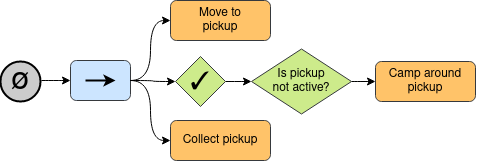
\includegraphics[scale=0.5]{Images/images/PickupMovement.drawio.png}} 

\subfloat[\centering Camera and guns]{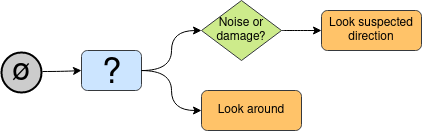
\includegraphics[scale=0.5]{Images/images/PickupHead.drawio.png}}
\caption{Behaviour Trees governing the actions of the bot collecting a pickup}
\label{fig:pickup_bt}
\end{figure}

When running low on health or ammo, a bot might decide to switch to the \textbf{Collect pickup state} (\Cref{fig:pickup_bt}) in order to collect the med-kits and ammo crates scattered through the map.

The score assigned to this state is computed as the maximum score assigned to all pickups in the map.

The bot calculates the score of each pickup based on the following factors:

\begin{itemize}
\item Absolute value of the pickup: Pickups that restore a higher amount of health or ammo are given higher scores.
\item Relative value of the pickup: The bot takes into consideration its current health and ammo levels and values pickups more highly the lower its current levels are.
\item Proximity to other pickups: Pickups located close together are given higher scores as they can be collected more efficiently.
\item Time to collect pickup: Pickups located closer to the bot's current position are considered safer and more valuable as they can be collected quicker.
\item Uncertainty of the pickup status: If the bot is uncertain about the availability of a pickup, it is considered a higher risk and given a lower score.
\end{itemize}

Once the pickup to collect is chosen, the bot will compute the shortest path to reach it and start moving towards it, while keeping an eye open for danger. This is achieved by looking around and turning immediately in case noise was heard or damage was received.
Once the correct location of the pickup is reached, the bot will remaining in the area, waiting for it to respawn if needed, and then proceed to collect it.

One important thing to notice is that the bot knowledge is continuously being updated, so at any time the score assigned to a pickup might change as a result of new information acquired and, consequently, the score assigned might change, potentially resulting in switching the pickup to collect.

As an example for this, imagine that the bot was headed to collect a pickup which believed to be active but, upon reaching its location, discovered it wasn’t. If another pickup is close by, the bot might decide to avoid waiting for the currently selected one to respawn and instead opt to fetch the other one.

\subsubsection{Search enemy}
\begin{figure}
\centering
\captionsetup[subfigure]{}
\subfloat[\centering Movement]{
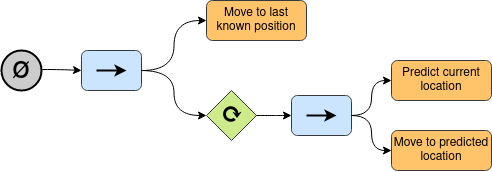
\includegraphics[scale=0.5]{Images/images/SearchMovement.drawio.png}} 

\subfloat[\centering Camera and guns]{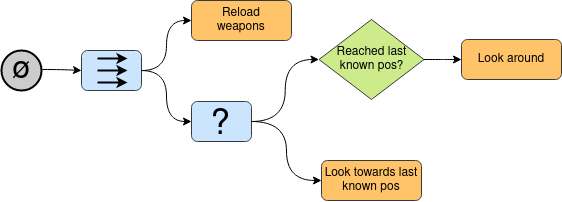
\includegraphics[scale=0.5]{Images/images/SearchHead.drawio.png}}
\caption{Behaviour Trees governing the actions of the bot searching an enemy}
\label{fig:search_bt}
\end{figure}

Any time the bot hears a suspicious noise or receives damage when the enemy position is unknown or otherwise when the enemy status switches from \textit{Detected} to \textit{Lost} (See \Cref{subsubsection:target_knowledge_base}), its possible for the bot to decide to switch to the \textit{Search Enemy state}, shown in \Cref{fig:search_bt}.

In this state, the first thing the bot will do is to try to reach the last known enemy position, which might be exact, if the enemy was seen standing there, or an approximation, if the enemy was only heard or damage came in from a specific direction. While reaching that destination, its important to keep the camera focused on that point, since the enemy might still be there. 

Once reached that position, the bot will need to fan out and search the area. This is normally done by simply choosing a random point to move to within a certain radius or the current position; however, given that skilled players are often able to predict the enemy location with a certain degree of accuracy, our bot has a probability of exactly pin-pointing the enemy current position. While reaching the new estimated position, the bot will look around as usual and, once reached destination, will try to guess again the enemy position.

During this entire process, the bot might randomly start to reload weapons if needed, in order to be ready for the possible upcoming fight.

Searching for the enemy continues until enough time passes or, in general, until the bot considers continuing the investigation favorable, after that the bot will switch its state to pursue another objective.

\subsubsection{Fight}

%TODO Put in horizontal page?
\begin{figure}
\centering
\captionsetup[subfigure]{}
\subfloat[\centering Movement]{
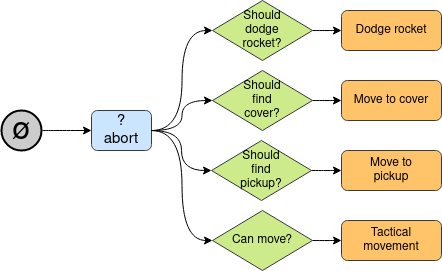
\includegraphics[scale=0.45]{Images/images/FightMovement.drawio.png}} 

\subfloat[\centering Camera and guns]{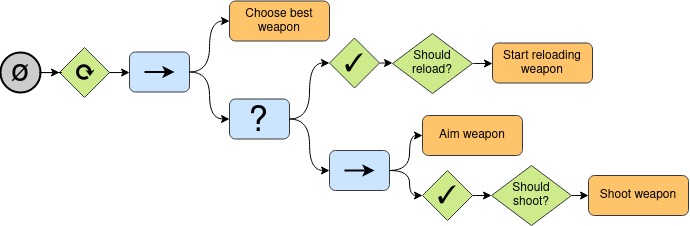
\includegraphics[scale=0.45]{Images/images/FightHead.drawio.png}}
\caption{Behaviour Trees governing the actions of the bot fighting an enemy}
\label{fig:fight_bt}
\end{figure}

A bot enters the \textit{Fight} state whenever it detects the enemy and is in a good enough shape to be able to likely survive the combat.
Correctly handling a fight is a complex process in which the bot must carefully orchestrate how to move, where to move, what weapon should be used, when should it be used or reloaded, as shown in \Cref{fig:fight_bt}.

\paragraph{Movement}\mbox{}\\
For what concerns movement, we identified 4 different objectives:

\begin{enumerate}
\item \textbf{Dodge rockets}: If the bot sees any incoming explosive projectile, it should try to distance itself from the missile and the blast it will cause.
\item \textbf{Find cover}: whenever the bot is running out of ammo and switching weapon might not be convenient, there is a random chance (to avoid predictable behaviors) it might consider moving behind cover to safely reload. If so, the bot find any position from which the enemy cannot see it, move towards that location and stay there until it has finished reloading. If at any point the cover should stop being valid, a new cover point will be selected.
\item \textbf{Collect pickup}: Whenever a useful pickup is close by, the bot can decide go fetch it without abandoning the fight (by avoiding to switch to the Collect pickup state). 
\item \textbf{Keep distance}: The bot will move around trying to try to keep the optimal distance from the enemy based on the currently equipped weapon and, if possible, will try to keep the enemy is sight. More skilled bots will try to circle strafe\footnote{Circle strafing is the technique of moving around an opponent in a circle while facing them. Circle strafing allows a player to fire continuously at an opponent while evading their attacks.} the enemy to gain the upper hand in the fight.
\end{enumerate}

The objective above are ordered by priority, so, for example, dodging rockets will always be preferred over collecting a pickup and, should the enemy fire with such projectile in our direction, we will abort fetching whatever object we wanted to try and dodge the incoming missile.

\paragraph{Gun selection}\mbox{}\\
A bot that simply moves during fight doesn’t achieve much, so for what concerns fighting back the process starts by choosing the optimal weapon to equip.

The gun selection process of the bot involves evaluating two key factors: the distance to the enemy and the amount of available ammo. Based on these parameters, the bot chooses the best weapon for the current combat situation, taking into account the optimal range of each weapon and avoiding, if possible, weapons that require reloading, since it might take a while before the bot is able to use them once equipped. The weapon scored higher according to these criteria is immediately equipped and will be used until another, more suitable weapon, should be chosen instead.

\paragraph{Aiming model}\mbox{}\\
Following the selection of the optimal gun, the bot should try to aim at the target. Although the concept of aiming for a bot is straightforward (just align the cross-hair to the enemy), achieving realistic aiming is more challenging. To account for human-like reaction times and aiming errors, the bot implements a modified version of Arnaboldi's aiming model based on "reflex" and movement predictability, described in \citep{arnaboldi_framework}. 

The bot aims at the enemy's predicted position, taking into account two types of \textit{aiming delays}: an uncorrectable delay and a correctable delay. The correctable delay can be compensated by considering the target's average position in the past. This means that enemy bots with predictable movement patterns will be easier to target than those with erratic movements.

In order to obtain an enemy position and average velocity at a given time, the \textit{Position Tracker} component is used. A \textit{Position Tracker} keeps track of the position of an entity  for every frame in the game up to a given number of seconds in the past. This list of position can be queried to extract both the bot position at a specific time and the bot average velocity in a given range, weighted in order to give less and less importance to velocities far away in time using \Cref{eq:average_velocity}.

\begin{equation}
\overline{v} = \frac{\sum_{i=1}^{n} v_i \cdot \left( W^{t_{end,i} - T_{f}} - W^{t_{start,i} - t_{TF}} \right)}{ \left( W^{T_{f} - T_{i}} \right)} 
\label{eq:average_velocity}
\end{equation}

Where:
\begin{itemize}
\item[$T_i$] The begin of the time range considered.
\item[$T_f$] The end of the time range considered.
\item[$n$] The number of frames for which we recorded position data in the time range considered. Each frame represents an interval of time.
\item[$v_i$] is the velocity in the interval $i$\footnote{Computed as the difference of position between two consecutive frames and the duration between them with the formula: $v_i = \frac{p_{t_{end,i}} - p_{t_{start,i}}}{t_{end,i} - t_{start_i}}$
}
\item[$W$] The weight parameter, the higher it is, the less weight is given to old speeds.
\end{itemize}

In addition to the \textit{aiming delays}, bots have also an \textit{aiming error}: a simple angle representing the deviation from the desired aiming position and the actual one.

\subsubsection{Actuator layer}
%TODO
Every kind of interaction that the bot wants to perform in the virtual world must be processed by the \textit{Actuator layer}, which is currently responsible of moving the bot, rotating the camera or shooting, reloading and switching weapons as a response to what action plan the \textit{decision layer} is currently following.

\subsection{Bot parametrization and profiles}
To emulate different types of human players with varying skills and attitudes, the bot capabilities and behaviors are determined by a set of parameters.

These parameters follow the same principles introduced by Arnaboldi in Cube 2\cite{arnaboldi_framework}, so we defined a \textit{general ability level} affecting all the bot capabilities, and more specific skills that determine a bot proficiency in a particular area compared to other bots with the same general ability level.
In general, the final value for a skill is computed as:

\begin{equation}
skill\_value = min(ability\_score * skill\_score, 1.0)
\label{eq:skill_value}
\end{equation}

The specific characteristics we identified are:
%TODO better ordering
\begin{itemize}
\item \textit{Eye speed}: Determines the maximum camera rotation speed and acceleration. Higher values allow bots to more quickly look in any direction, giving them advantages in scouting an area or aiming at a target.
\item \textit{Reflexes}: Determines how quickly an entity reacts to inputs from the outside world, such as sound for a gun firing, receiving damage or seeing an enemy. 
\item \textit{Prediction skill}: Determines how proficient a bot is in tracking down a lost enemy. Higher values ensure that a bot is more likely to correctly predict an unseen enemy current location.
\item \textit{Aiming skill}: Determines how big the aiming delays and errors are on average, therefore influencing the accuracy of the bot.
\item \textit{Speed}: Determines the movement speed of a bot\footnote{For the purpose of our research, all bots are given the same speed.}.
\item \textit{Movement skill}: Determines how good the bot is in moving tactically when fighting. Higher values ensure a bot employes advanced techniques such as strafing\footnote{Circle strafing is the technique of moving around an opponent in a circle while facing them. Circle strafing allows a player to fire continuously at an opponent while evading their attacks}.
\item \textit{Curiosity}:  The frequency with which the bot looks around instead of solely forward.
\item \textit{Recklessness}: Determines how aggressiveness of the bot. At higher values, a bot will tend to favour combat above everything else, while at low value a bot will prefer finding cover and retreating when in danger.
\item \textit{Field of view}: Determines the field of view of the bot.
\item \textit{Max view range}: The maximum distance an item or enemy can be seen.
\end{itemize}

Using these characteristics, we defined three different bot profiles that will be used in our experiments:
\begin{itemize}
\item \textbf{Shotgun}: The \textit{Shotgun} profile represents a bold and aggressive player who is always ready for a fight. This bot excels in movement, able to quickly close the gap between it and its enemy in order to overpower it in close-quarters combat using its shotgun.
\item \textbf{Sniper}: The \textit{Sniper} profile represents a calculated and patient player who excels in long-range combat. This bot possesses exceptional aiming skills with its sniper rifle, allowing it to take out enemies from a distance with deadly accuracy. It prefers to avoid direct confrontation whenever possible and instead chooses to pick off its enemies from a safe distance. 
\item \textbf{Assault}: The \textit{Assault} profile represents a versatile and well-rounded player who is skilled in both short and medium-range combat. This bot is equipped with an assault rifle.  
\end{itemize}

In \Cref{table:1} the different skills scores for each profile are presented.

%TODO same ordering as above
\begin{table}
\begin{center}
\begin{tabular}{|| c || c | c | c ||}
 \hline
 Skill & Shotgun & Assault & Sniper \\ 
 \hline 
 Eye speed & 1.2 & 1 & 0.8 \\  
 Reflex & 0.9 & 1 & 1.3 \\   
 Prediction & 1.1 & 1 & 0.7 \\  
 Aim & 0.6 & 1 & 1.15 \\  
 Movement & 1.2 & 1 & 0.6 \\  
 Curiosity & High & Neutral & Low \\  
 Recklessness & High & Neutral & Low \\  
 MaxRange & 50 & 120 & 200 \\  
 Speed & 20 & 20 & 20 \\  
 \hline
\end{tabular}
\caption{Different bot profiles defined for our experiments}
\label{table:1}
\end{center}
\end{table}

\section{Summary}
In this chapter we gave a brief overview of Ballabio's Unity Framework, on top of which we built our work.

We then briefly described the kind of data that the framework can gather and analyse during simulation to support any kind of experiment.

Finally, we analyzed the bot system we created to help us run simulations, focusing on its structure and components, how information flows between them, how it makes decisions, what are the parameters governing its decisions and actions and how they can be configured to better represent specific player's capabilities and play styles.